
 \begin{figure*}[ht]
    \centering
    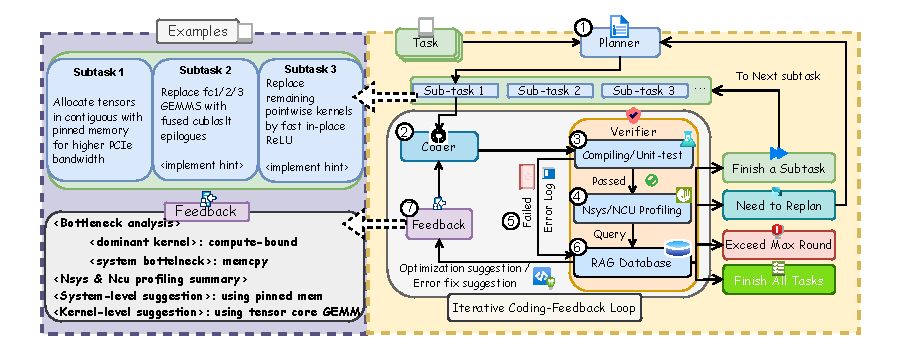
\includegraphics[width=\linewidth]{pic/main-workflow.pdf}
    \caption{StitchCUDA: \textcircled{1} The Planner profiles the reference implementation using Nsys to identify performance bottlenecks and generates a structured to-do list of optimization tasks.
\textcircled{2} The Coder executes one subtask per iteration,
\textcircled{3} compiles the modified code with \texttt{nvcc}, and produces an executable for unit testing.
\textcircled{4} The Verifier selects the appropriate profiling tool (Nsys, NCU, or both) to analyze the target kernel.
\textcircled{5} If compilation/correctness fails, the profiling stage is skipped.
\textcircled{6} Relevant  Nvidia's official documentation is retrieved via a RAG module, and
\textcircled{7} Construct a single task feedback to Coder to initiate the next coding-feedback iteration.}
    \label{fig:main}
    \vspace{-5pt}
\end{figure*}
\section{Framework Design and Methodology}
To effectively scale multi-agents system to end-to-end GPU programming, we present StitchCUDA, a multi-agent framework composed of three agents. Planner, Coder, and Verifier that jointly perform iterative optimization of end-to-end GPU programs. The Coder agents are further enhanced with rubric-based agentic RL to improve their responsiveness to feedback from Verifier, enabling more effective self-correction and optimization over iterations. In this section, we will discuss in detail our multi-agent design and the method in rubric-based agentic RL for Coder.

\subsection{Multi-agent Framework Workflow}
\label{sec:multi_agent_workflow}
StitchCUDA orchestrates specialized agents with a global state machine that shares a typed \texttt{State}, containing generated code, profiling artifacts, and routing decisions. The workflow is an Iterative Coding-Feedback Loop, as shown in Fig.\ref{fig:main}. The details of each agent are below:

\vspace{-10pt}
\begin{itemize}
\item \textbf{Planner}: parses the reference PyTorch code, builds a minimal profiling harness, and records Nsys traces to identify time-dominant kernels and system hotspots. The agent then emits a structured to-do list with task identifiers, target kernels, expected shapes, and constraints (e.g., data types or numeric tolerance) that guide downstream code generation. Using chain-of-thought prompting, the Planner reasons at the system level to decompose the workload into subtasks that jointly consider kernel-level efficiency and host-side orchestration, improving the feasibility and coherence of the generated plan.

\item \textbf{Coder}: generates CUDA implementations for the current subtask in a self-contained project (source, build files, Pybind interface) and invokes
\texttt{nvcc} to compile. It writes kernel stubs and launch code, host-side orchestrations that match the Planner's spec, and captures build artifacts (executable path, logs, and generated source) in the shared \texttt{State}. After receiving the Verifier's feedback with optimization suggestions, the Coder refines the current subtask accordingly.

\item \textbf{Verifier}: validates correctness and performance. When compilation fails, it analyzes the error log and returns concrete fix guidance for the Coder (e.g., missing headers, signature mismatches, or type errors). When tests pass, the Verifier analyzes the end-to-end program from two perspectives, using Nsys first identifies the dominant GPU kernel that costs the most GPU time and dominant system-level bottlenecks (e.g., data transfer between CPU and GPU, kernel launch, CPU-GPU synchronization). It then profiles the identified bottleneck kernel with NCU. First, it classifies it as memory-bound or compute-bound and automatically selects relevant performance metrics for detailed analysis. Based on this two-level diagnosis, the Verifier produces actionable optimization suggestions addressing both kernel-level improvements and required system-level changes, which are routed back to the Planner or Coder.
\end{itemize}

In addition, we prepare several up-to-date CUDA/GPU documents (e.g., the white paper of Hooper and Blackwell GPUs, the newest tutorial of CUBLAS/CUTLASS library) for Planner and Verifier to use Retrieval-Augmented Generation \cite{lewis2021retrievalaugmentedgenerationknowledgeintensivenlp} in inference, so that they can provide effective plans and optimization feedback, combining with the newest hardware specs and software stacks. Details about RAG implementations are shown in Appendix~\ref{app:rag}.

Verifier routes the whole loop based on tests' outcomes: attempt the task again if failed, further optimize current task for better performance if successful, then advance to the next task on success and good speedup; replan when fundamental mismatches are detected, overall final test performance is slower than reference; stop when the iteration budget is exhausted. The detailed prompts for every agent are shown in Appendix~\ref{app:prompt}.

\begin{figure*}[ht]
    \centering
    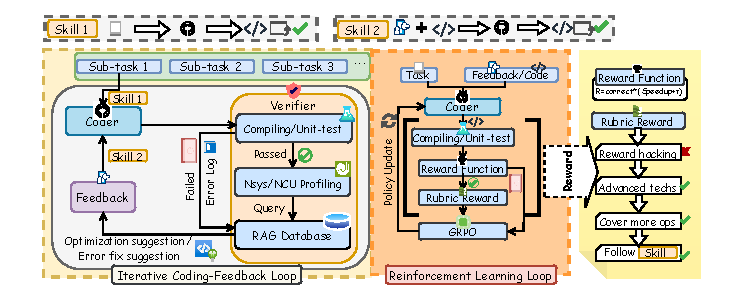
\includegraphics[width=\linewidth]{pic/RL.pdf}
    \caption{Rubric-based Agentic RL process for Coder. We train the Coder on two atomic skills via GRPO. Besides the rule-based reward function, we introduce a rubric reward to avoid reward hacking and encourage more kernel optimizations.}
    \label{fig:RL}
    \vspace{-10pt}
\end{figure*}

\subsection{Rubric-based Agentic RL for Coder}





\subsubsection{Decomposing Multi-turn Interactive Trajectories into Atomic Skills}

To retain the benefits of agentic RL while avoiding prohibitive multi-turn
rollout cost (See~\ref{app:time}), we decompose the multi-turn agentic RL into learning two
\emph{atomic skills} that recur throughout our workflow (Fig.~\ref{fig:RL}):
\textbf{Skill~1}, generating CUDA kernels from reference PyTorch code and subtask
requirements; and \textbf{Skill~2}, improving an existing kernel by following
feedback and implementing targeted optimizations. We then train these skills in
a single-turn RL.

Concretely, for Skill~1, we sample 80\% of tasks from KernelBench Levels~1--3 and
use a Planner to produce subtasks. After filtering with human
experts, we obtain 200 curated samples containing reference PyTorch code, subtask
requirements, and prompt templates. For Skill~2, we run our framework on the
same tasks, using Qwen3-32B as the Coder to collect verifier feedback, and retain
only feedback instances that lead to a correct next-iteration kernel. This
yields 200 additional samples containing previous code, feedback, and reference PyTorch code. Finally, we merge those samples and apply GRPO to jointly
optimize the Coder across the two skills, providing an efficient surrogate for
multi-turn RL without high rollout overhead.

\subsubsection{Using Rubric Reward for RL Training}

To mitigate reward hacking/degenerate behaviors and encourage more optimization,
we introduce a \emph{Rubric Reward} that provides a comprehensive
assessment of candidate kernels. Rubric-based rewards are commonly used to
evaluate attributes that are not fully captured by simple tests or scalar
metrics~\cite{huang2025reinforcementlearningrubricanchors,liu2026openrubricsscalablesyntheticrubric}.
Our rubric is designed and validated by human CUDA experts with assistance from
advanced LLMs, and scores each candidate along four dimensions: \textbf{(i)
Anti-Hacking}, penalizing reward exploitation; \textbf{(ii) CUDA Engineering},
rewarding advanced optimization techniques; \textbf{(iii) Operator Coverage},
encouraging broader optimization for complex multi-operation programs; and \textbf{(iv)
Skill Compliance}, enforcing adherence to task requirements (Skill~1) or feedback
instructions (Skill~2). Each dimension uses a discrete scale with detailed
criteria per score level. Concretely, we aggregate these scores into a
normalized shaping term:
\begin{equation}
\hat{r}_{\mathrm{rubric}}
=
\left[
\frac{
\sum_{k=1}^{K} s_k- K\,s_{\min}
}{
K\,(s_{\max}-s_{\min})
}
-\frac{1}{2}
\right],
\label{eq:rubric_reward}
\end{equation}
where $s_k \in \{1,\dots,5\}$ denotes the discrete score for the $k$-th rubric
criterion, $K$ is the number of rubric dimensions, and $s_{\min}=1$ and
$s_{\max}=5$ are the per-dimension bounds. This normalization maps the rubric
scores to a centered range, producing a stable shaping signal that complements
the rule-based reward. Details of reward design are in the Appendix~\ref{app:rubric}.













\paragraph{Final reward formulation.}
We combine rubric-based shaping with a rule-based reward function(based on correctness and speedup) to form the final training reward:
{\footnotesize
\begin{equation}
R
=
\mathbb{I}_{\mathrm{corr}}
\cdot
\bigl(1-\mathbb{I}_{\mathrm{hack}}\bigr)
\cdot
\min\!\left(
\left(s + \tau \right)
\left( 1 + \lambda\,\hat{r}_{\mathrm{rubric}} \right),
\; R_{\max}
\right),
\label{eq:final_reward}
\end{equation}
}
where $\mathbb{I}_{\mathrm{corr}} \in \{0,1\}$ indicates whether the generated
kernel passes the benchmark’s functional correctness verification.
$\mathbb{I}_{\mathrm{hack}} \in \{0,1\}$ flags major reward-hacking behaviors;
When $\mathbb{I}_{\mathrm{hack}}=1$, the reward is suppressed to prevent policy
updates from reinforcing exploitation. The scalar $s$ denotes the measured
runtime speedup over the reference implementation. The constant $\tau=0.3$
provides an additive offset to avoid vanishing rewards for correct kernels with
marginal speedup. The coefficient $\lambda=1$ controls the contribution of
rubric-based shaping relative to rule-based reward, and $R_{\max}=5$
caps the maximum reward magnitude to stabilize policy optimization and avoid training collapse.

\paragraph{Training details.}
We train the Coder under a single-turn setting using GRPO, targeting both
skills as described in the previous section. We adopt Qwen3-32B as the Coder backbone, as its strong reasoning capability alleviates sparse-reward and better matches the distribution of RL samples. In each training step, we sample a batch of 16 prompts and generate $8$ rollouts per prompt. We then compute the GRPO objective from~\cite{Guo_2025} and update the policy:

{\tiny
\begin{equation}
\resizebox{\linewidth}{!}{$\displaystyle
    \begin{aligned}
        \mathcal{J}_{\text{GRPO}}(\theta) 
        &= \mathbb{E}_{\substack{q \sim P(Q),  \{o_i\}_{i=1}^G \sim \pi_{\theta_{old}}(O|q)}} 
        \Bigg[ \frac{1}{G} \sum_{i=1}^G \frac{1}{|o_i|} \sum_{t=1}^{|o_i|} \\
        &\quad \min \bigg( 
            \frac{\pi_\theta(o_{i,t} | q, o_{i,<t})}{\pi_{\theta_{old}}(o_{i,t} | q, o_{i,<t})} \hat{A}_{i,t}, \\
        &\quad \text{clip} \left( 
            \frac{\pi_\theta(o_{i,t} | q, o_{i,<t})}{\pi_{\theta_{old}}(o_{i,t} | q, o_{i,<t})}, 1 - \epsilon, 1 + \epsilon 
        \right) \hat{A}_{i,t} 
        \bigg) \\
        &\quad - \beta \mathbb{D}_{KL} \left[ \pi_{\theta} \parallel \pi_{ref} \right] \Bigg],
    \end{aligned}$}
    \label{eq:GRPO-obj}
\end{equation}
}
where $\hat{A}_{i,t} = \frac{r_i - \mathrm{mean}(\mathbf{r})}{\mathrm{std}(\mathbf{r})}$,
$\mathbf{r}=\{r_i\}_{i=1}^{G}$ are the rollout-level rewards, and each $r_i$ is
computed using Eq.~\ref{eq:final_reward}, where we deploy Qwen3-32B to assign rubric reward. Training is conducted on 4 H200 GPUs. We set \texttt{max\_response\_length} to 16384 and use LoRA for compute-efficient fine-tuning with \texttt{rank}$=$\texttt{alpha}$=$128. The sampling parameters follow the Qwen3 Team~\cite{qwen3technicalreport}. Training one Coder costs approximately 20 Hours.




\label{RLdesign}